\chapter{システム実験の詳細}
システム実験では全三回にわたる実験を行い、被験者同士の対戦を行う第三回以外の二回は被験者がAIとの対戦とAIを用いた振り返りを行う。
第四章と同様に3回1セットの実験のうち、前半二回を第一段階・後半一回を第二段階と呼ぶ。
以下で実験設定や結果の詳細を段階ごとに述べていく。
\section{第一段階}
第一段階はAIとの対戦とその振り返りによって構成されている。
振り返りモードでは表示する予想図の手数、AIの強さを被験者ごとに変更しつつ実験を行った。
予想図の手数は$\{3, 5, 7, 制限なし(最後まで表示)\}$の4段階、AIの強さは$\{強,弱\}$の2段階を設定した。
使用したAIモデル(alphazero\_baseline),提案手法に与えるパラメータを表\ref{table:param-system}に示す。
\begin{table}[H]
	\caption{AIモデルのパラメータ(システム実験・第一段階)}
	\centering
	\scalebox{0.98}[0.98]{
		\begin{tabular}{c|c|c}
			モデル&強&弱\\\hline
			time    & 5 & 1 \\ 
			$C_{puct}$ & 1   & 0.25 \\
			$k$ (提案手法のみ)     & 4 & 4 \\
			$l$ (提案手法のみ)     & 2 & 2 \\

		\end{tabular}
	}
	\label{table:param-system}
\end{table}
また、1回の実験当たりの制限時間は7分とし、実験内のAIとの対戦は2回までに制限した。
これは実戦経験による熟達ではなく支援システムによる学習過程の観察という実験の趣旨に従うためである。
\subsection{振り返りモード(GUI)の詳細}
振り返りモードでは直前の対戦の内容を振り返ることができる。
「>/<」ボタンを押すことで「一つ先の盤面に進む/戻る」ことができる。
また、振り返りを補助する機能として画面左下の「counts」に表示されている盤面$s$に対する
各行動の訪問回数$N(s)$,「value」に局面評価$V(s)$を示した。
$N(s),V(s)$は対戦に使用したモデルから導かれる。
数字が書かれているボタンはAIモデル(対戦に使ったモデルと同じ)による予想図を提示するボタンであり、ボタンに描かれた数字
と同じ列を選択した場合の予想図を見ることができる。
図\ref{fig:number-button}では「4」と描かれたボタンを押した結果、左から4番目を選択した場合の予想図が表示されていることがわかる。
選択した位置は「\*」マークで表示される。
\begin{figure}[t]
	\centering
	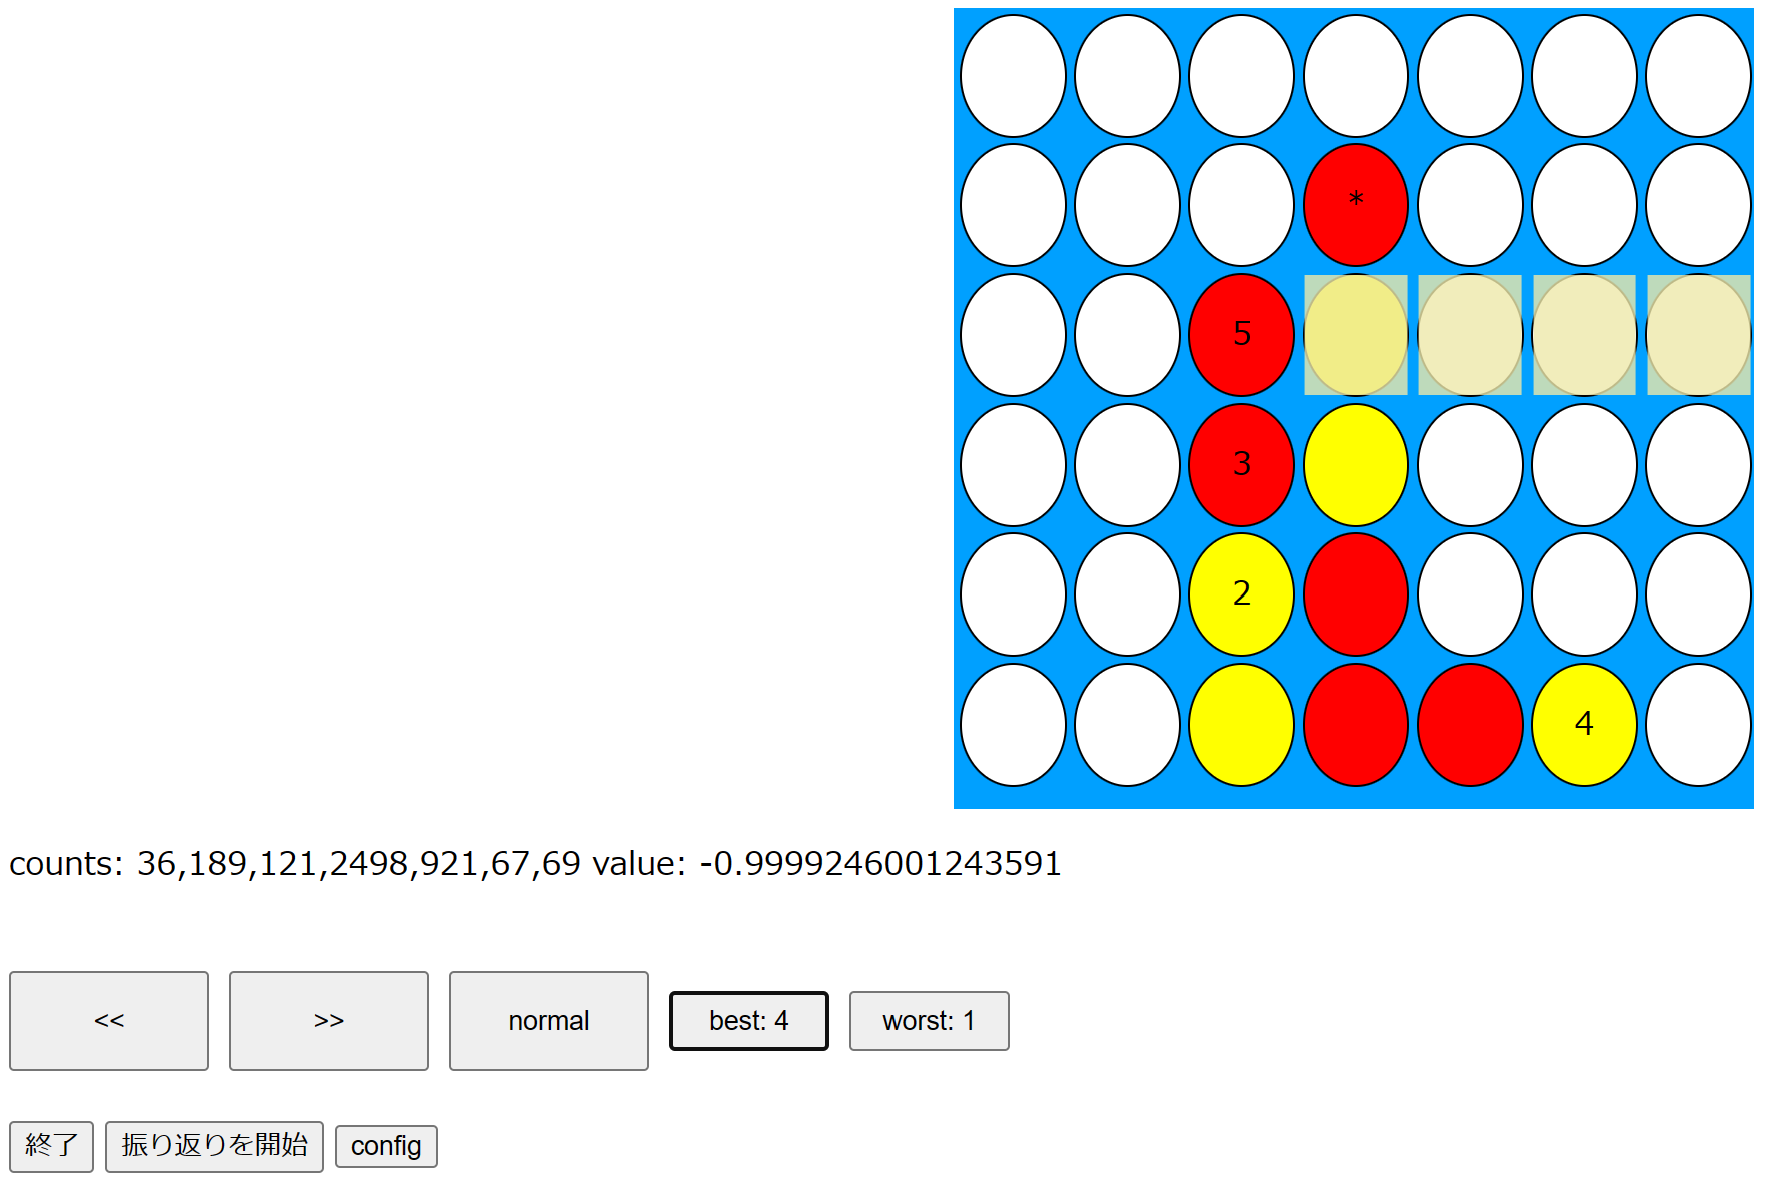
\includegraphics[width=\linewidth]{./figure/trajSystem.png}
	\caption{予想図の提示}
	\label{fig:number-button}
\end{figure}
想定図中の数字は数字の大きさの順番に石が置かれるというAIの予想を表している。図\ref{fig:number-button}
では赤が「\*」マークの位置に石を置いた次に黄は左から3列目の位置、その次に赤は左から3列目に打つことが予測されている。
また、図中で色づけられている部分は予想図においてその部分がは四つ以上つながることを示している。赤く色づけられている場合はその部分で
赤が4つ以上つながると予想されていること、黄色く色づけられている場合はその部分で黄色が4つ以上つながると予想されているこを示している。
また、提案手法による振り返りが適用されたグループでは提示される予想図が複数となる。そのため図\ref{fig:multi}に示すように他の想定図を見ることができる「next\_prej/pre\_traj」
が追加される。
\begin{figure}[t]
	\centering
	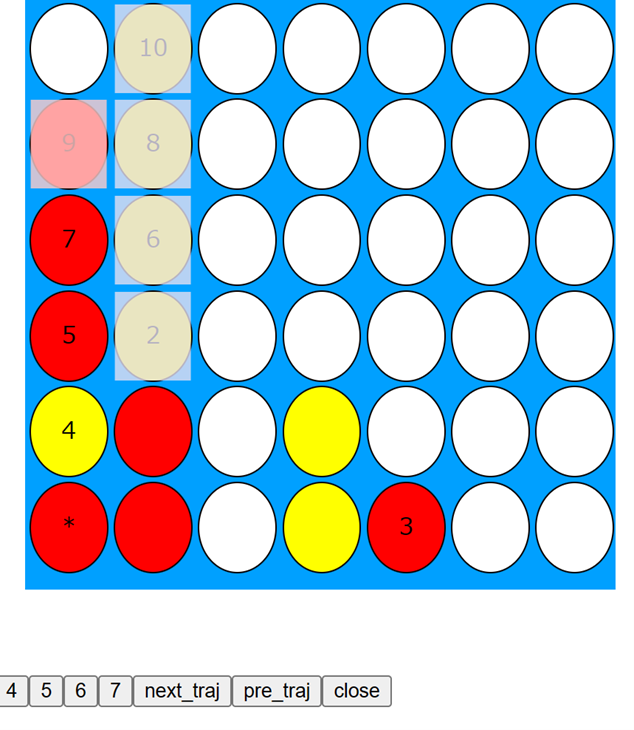
\includegraphics[width=\linewidth]{./figure/multi.png}
	\caption{提案手法による予想図の提示}
	\label{fig:multi}
\end{figure}
ここからは第一段階中の一日目、二日目のGUIの違いについて述べる
\subsection{一日目}
一日目は被験者の操作間への慣れを促進するため全ての選択肢に対して予想図表示ボタン(数字ボタン)を設置した。
図\ref{fig:traj-button}に示すようにこれらのボタンは「traj」ボタンを押すことで出現する。
\begin{figure}[t]
	\centering
	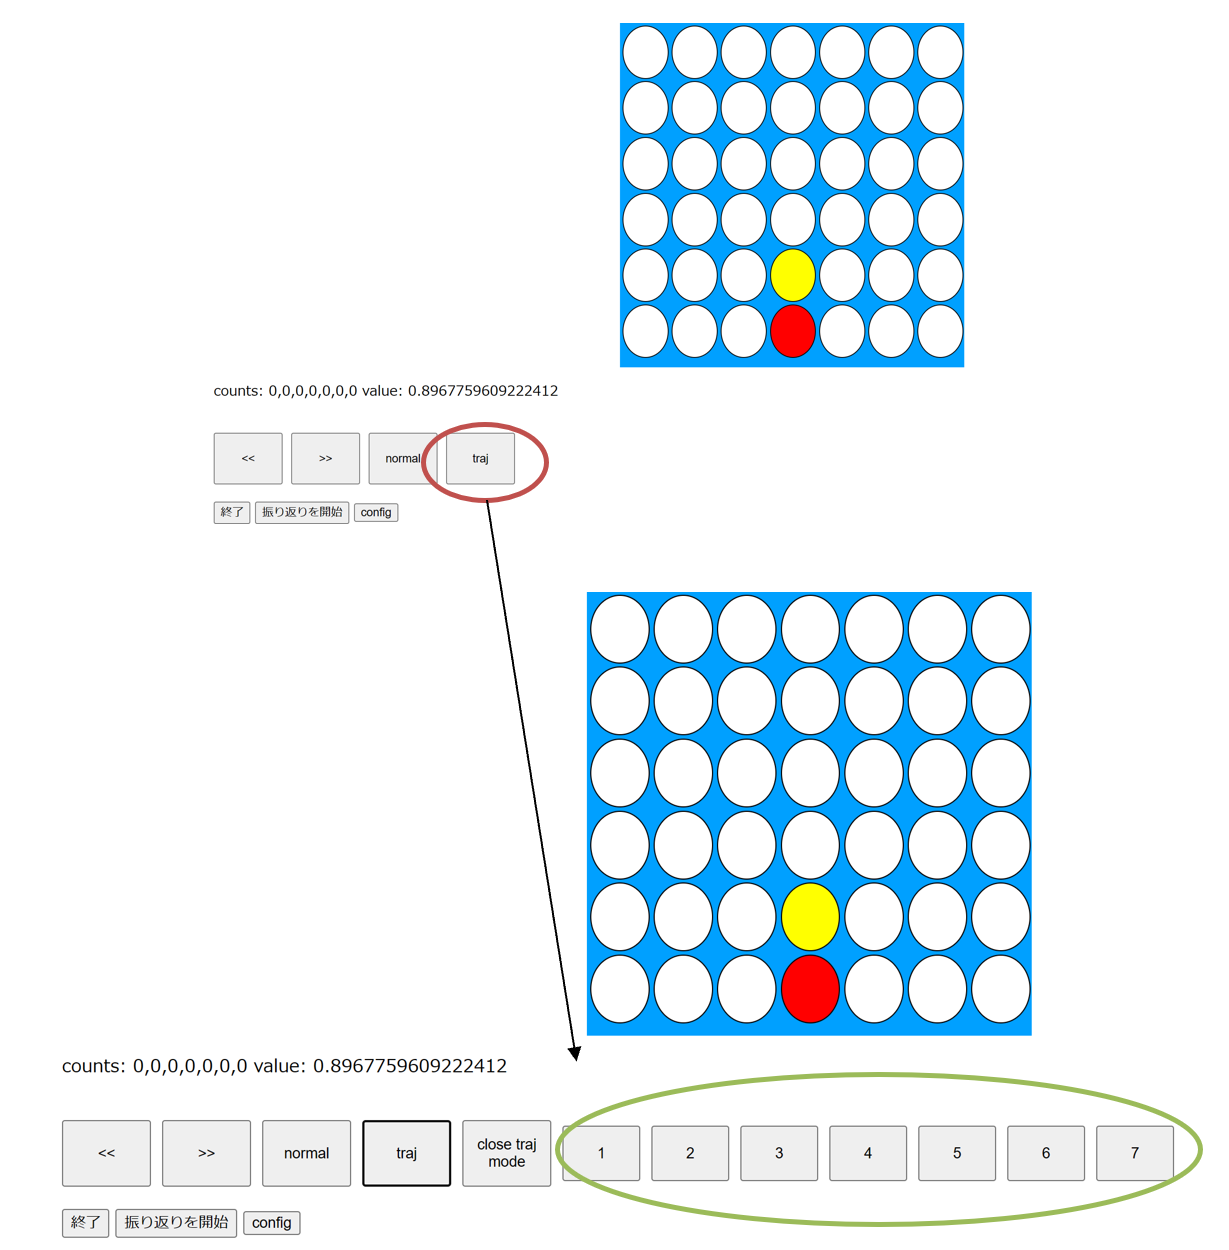
\includegraphics[width=\linewidth]{./figure/traj-button.png}
	\caption{予想図表示ボタン(一日目)}
	\label{fig:traj-button}
\end{figure}
\subsection{二日目}
二日目は予想図の閲覧を促進するためtrajボタンを廃止し、最も訪問回数$N(s,a)$の多い選択肢$a_{max}$,少ない選択肢$a_{min}$
からの予想図を示すボタンをそれぞれ「best:(列の数字)」「worst:(列の数字)」のラベルで図\ref{fig:best-worst}のように表示した。
\begin{figure}[t]
	\centering
	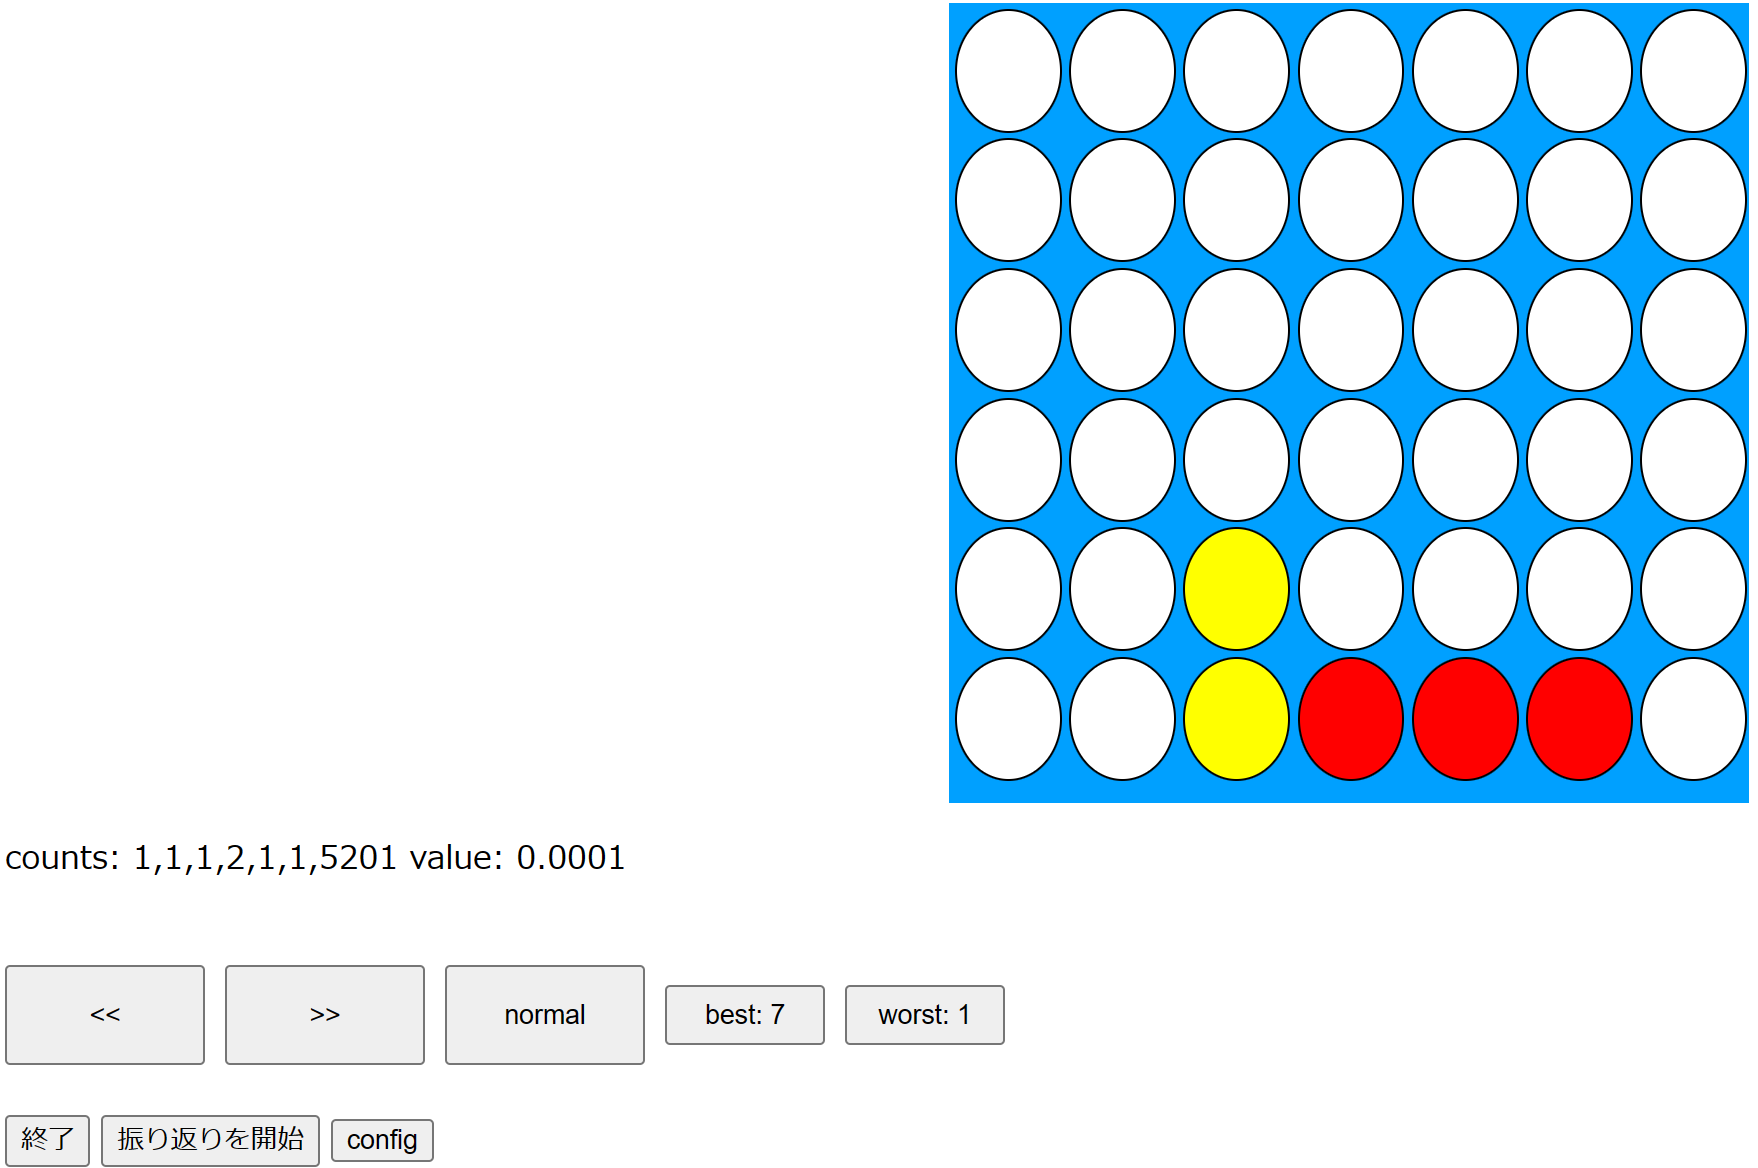
\includegraphics[width=\linewidth]{./figure/best-worst.png}
	\caption{予想図表示ボタン(二日目)}
	\label{fig:best-worst}
\end{figure}
\section{第二段階}
第二段階は提案手法を用いて振り返りを行ったグループ(A)の被験者と比較手法を用いて振り返りを行ったグループ(B)の被験者の対戦である。
一回の実験の中で二人の被験者が手番を入れ変え二回の対戦を行った。
制限時間は1ゲーム5分であり、制限時間内に終わらなかったゲームはAIによって判定した。具体的には制限時間が切れた際の盤面$s$のAIによる局面評価$V(s)$の絶対値が0.5以上である場合に
はその符号が示すプレイヤーの勝利とし、$V(s)$の絶対値が0.5未満である場合は引き分けとする。
判定用に使用したAIモデルのパラメータは\ref{table:param-judge}に示す。
\begin{table}[H]
	\caption{AIモデルのパラメータ(システム実験・第二段階)}
	\centering
	\scalebox{0.98}[0.98]{
		\begin{tabular}{c|c}
			パラメータ名 & 値 \\ \hline
			time    & 0\\ 
			$C_{puct}$    & 1 \\
		\end{tabular}
	}
	\label{table:param-judge}
\end{table}


\section{質問項目の詳細}
質問項目は「タスクの熟達度に関連する質問」と「タスクの楽しさ・面白さに関連する質問」の二つに分けられる。
具体的な質問項目は\ref{table:query}に記載した。また、二日目は「タスクの楽しさ・面白さに関連する質問」に
「一回目と比べて成長したと感じますか」を追加した。
\begin{table}[H]
    \caption{質問項目:システム実験}
	\scriptsize
    \begin{tabular}{c||l}
        \multicolumn{1}{c|}{質問の種類} & \multicolumn{1}{c}{質問の内容} \\ \hline \hline
        \multicolumn{1}{c||}{}&対局によって成長したと感じましたか \\
        タスクの熟達度に関連する質問 & 振り返りによって成長したと感じましたか \\
		\multicolumn{1}{c||}{}&振り返りによってAIの意図を掴むことができたと感じますか \\
		\multicolumn{1}{c||}{} & (二日目のみ)一回目と比べて成長したと感じますか\\\hline
        \multicolumn{1}{c||}{} & 今後もconnect4をプレイするときにこのシステムを使いたいと思いましたか \\
        タスクの楽しさ・面白さに関連する質問 & システムにより振り返りが楽しくなったと感じますか\\
    \end{tabular}
    \label{table:query}
\end{table}



